% Mirror: https://github.com/SIGma-UIUC/presentation-format
% --------------------------------------------------------------------
% This is a simple Beamer document that uses beamerthemesigma.sty
% Reading the comments should help you create a presentation even if
% you've never used Beamer before.
% --------------------------------------------------------------------

% Set our document class to Beamer
\documentclass[aspectratio=169]{beamer}
% \documentclass[aspectratio=169, handout]{beamer}
% Add handout option to ignore pauses

% From Jeff E
\usepackage{algo}
% Some more macros
\usepackage{sigmastyle}
% Diagrams
\usepackage{tikz}
\usetikzlibrary{matrix}

% Set a title
\title{Fibonacci Heaps}

% Set a subtitle if you desire
\subtitle{}

% Whoever worked on the presentation:
\author{Porter Shawver}

% Date looks ugly, so leave blank
\date{}

% An institute name, if you're so inclined
% \institute{University of Illinois Urbana-Champaign}

% Use the SIGma theme for this Beamer presentation
\usetheme{sigma}
% --------------------------------------------------------------------

% Begin document
\begin{document}

% Beamer calls each slide a "frame", defined within the environment:
% \begin{frame}
%   <frame content here>
% \end{frame}

% This frame is just the title.
\begin{frame}
\titlepage
\end{frame}

\begin{frame}{Come Make Meetings!}
    Brand New: \emph{Short and Sweet Presentations} \pause
    \begin{itemize}
        \item 3 presentations each day
        \item 10-15 minutes long (\emph{Short})
        \item Probably some food and drink (\emph{Sweet})
        \item March 18th \& April 22nd
        \item Good way to show you are interested in being a future admin
    \end{itemize} \pause
    Join Discord (\href{https://www.cstheory.org/discord}{cstheory.org/discord}) + DM any @admin if interested
\end{frame}

% A frame with the table of contents.
% This frame's title is "Outline".
\begin{frame}{Outline}
  \tableofcontents
\end{frame}


% Start a section: *sections* (subsections, etc.) are what show up in the TOC.
\section{Priority Queue Background}
% Section pages can be printed thus:
\frame{\sectionpage}
% There's a way to automate this, see:
% https://tex.stackexchange.com/questions/178800/creating-sections-each-with-title-pages-in-beamers-slides/178803

\begin{frame}{Priority Queues}
    For the entirety of this presentation, I will be using minimum priority queues, but maximum priority queues are implemented the same way.

    Operations:
    \begin{itemize}
        \item \textsc{Insert} - add an element to the queue.
        \item \textsc{FindMin} - return the smallest element.
        \item \textsc{DeleteMin} - remove the smallest element.
        \item \textsc{DecreaseKey} - decrease an element.
    \end{itemize}
\end{frame}


\begin{frame}{Binary Heap}
    A binary heap is a binary tree that maintains two properties:
    \begin{enumerate}
        \pause
        \item All children must have a value greater than their parent (``heap property''). Thus, the root should be the next value out of the queue.
        \pause
        \item The tree is complete (every level must be completely full, except the last). This allows us to use an array, and helps with worst case runtime.
    \end{enumerate}
\end{frame}

\begin{frame}{Binary Heap Example}
    \begin{center}
        \begin{tikzpicture}[%level distance=5mm,
            inner sep=2pt,
            every node/.style={draw,circle,minimum size=4ex},
            level/.style = {sibling distance = 50mm/##1},
            ]

            \node {7}
                child {node {15}
                    child {node {17}
                        child {node {31}}
                        child {node {24}}
                    }
                    child {node {19}
                        child {node {25}}
                        child {node[dashed, color=gray] {} edge from parent[dashed, color=gray]}
                    }
                }
                child {node {8}
                    child {node {16}
                        child {node[dashed, color=gray] {} edge from parent[dashed, color=gray]}
                        child {node[dashed, color=gray] {} edge from parent[dashed, color=gray]}
                    }
                    child {node {11}
                        child {node[dashed, color=gray] {} edge from parent[dashed, color=gray]}
                        child {node[dashed, color=gray] {} edge from parent[dashed, color=gray]}
                    }
                };
        \end{tikzpicture}
    \end{center}
\end{frame}


\begin{frame}{Binary Heap \textsc{Insert}}
    1. Add value to first open space.
    
    \begin{center}
        \begin{tikzpicture}[%level distance=5mm,
            inner sep=2pt,
            every node/.style={draw,circle,minimum size=4ex},
            level/.style = {sibling distance = 50mm/##1},
            ]
            
            \node {7}
                child {node {15}
                    child {node {17}
                        child {node {31}}
                        child {node {24}}
                    }
                    child {node {19}
                        child {node {25}}
                        child {node[color=red] {10} edge from parent[color=red]}
                    }
                }
                child {node {8}
                    child {node {16}
                        child {node[dashed, color=gray] {} edge from parent[dashed, color=gray]}
                        child {node[dashed, color=gray] {} edge from parent[dashed, color=gray]}
                    }
                    child {node {11}
                        child {node[dashed, color=gray] {} edge from parent[dashed, color=gray]}
                        child {node[dashed, color=gray] {} edge from parent[dashed, color=gray]}
                    }
                };
        \end{tikzpicture}
    \end{center}
\end{frame}
\begin{frame}{Binary Heap \textsc{Insert}}
    2. Swap with parent until the parent is smaller to maintain heap property.
    
    \begin{center}
        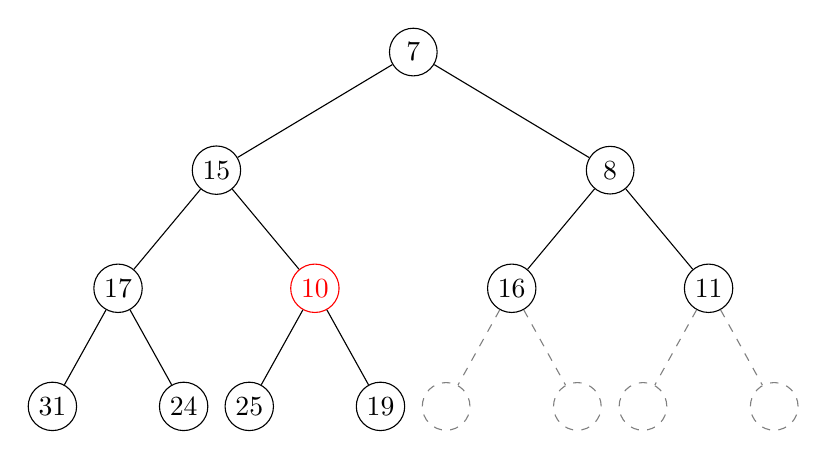
\begin{tikzpicture}[%level distance=5mm,
            inner sep=2pt,
            every node/.style={draw,circle,minimum size=4ex},
            level/.style = {sibling distance = 50mm/#1},
            ]
            
            \node {7}
                child {node {15}
                    child {node {17}
                        child {node {31}}
                        child {node {24}}
                    }
                    child {node[color=red] {10}
                        child {node {25}}
                        child {node {19}}
                    }
                }
                child {node {8}
                    child {node {16}
                        child {node[dashed, color=gray] {} edge from parent[dashed, color=gray]}
                        child {node[dashed, color=gray] {} edge from parent[dashed, color=gray]}
                    }
                    child {node {11}
                        child {node[dashed, color=gray] {} edge from parent[dashed, color=gray]}
                        child {node[dashed, color=gray] {} edge from parent[dashed, color=gray]}
                    }
                };
        \end{tikzpicture}
    \end{center}
\end{frame}
\begin{frame}{Binary Heap \textsc{Insert}}
    2. Swap with parent until the parent is smaller to maintain heap property.
    
    \begin{center}
        \begin{tikzpicture}[%level distance=5mm,
            inner sep=2pt,
            every node/.style={draw,circle,minimum size=4ex},
            level/.style = {sibling distance = 50mm/#1},
            ]
            
            \node {7}
                child {node[color=sigma@green] {10}
                    child {node {17}
                        child {node {31}}
                        child {node {24}}
                    }
                    child {node {15}
                        child {node {25}}
                        child {node {19}}
                    }
                }
                child {node {8}
                    child {node {16}
                        child {node[dashed, color=gray] {} edge from parent[dashed, color=gray]}
                        child {node[dashed, color=gray] {} edge from parent[dashed, color=gray]}
                    }
                    child {node {11}
                        child {node[dashed, color=gray] {} edge from parent[dashed, color=gray]}
                        child {node[dashed, color=gray] {} edge from parent[dashed, color=gray]}
                    }
                };
        \end{tikzpicture}
    \end{center}
\end{frame}
\begin{frame}{Binary Heap \textsc{Insert}}
    Worst case, the inserted value is the new smallest value, and must be swapped all the way to the top: \color{sigma@mainblue} $O(\log n)$.
\end{frame}


\begin{frame}{Binary Heap \textsc{FindMin}}
    The root is always the min, so finding it is \textcolor{sigma@mainblue}{$O(1)$}.
\end{frame}


\begin{frame}{Binary Heap \textsc{DeleteMin}}
    1. Return the root value, and replace the root node with the last element in the array.

    \begin{center}
        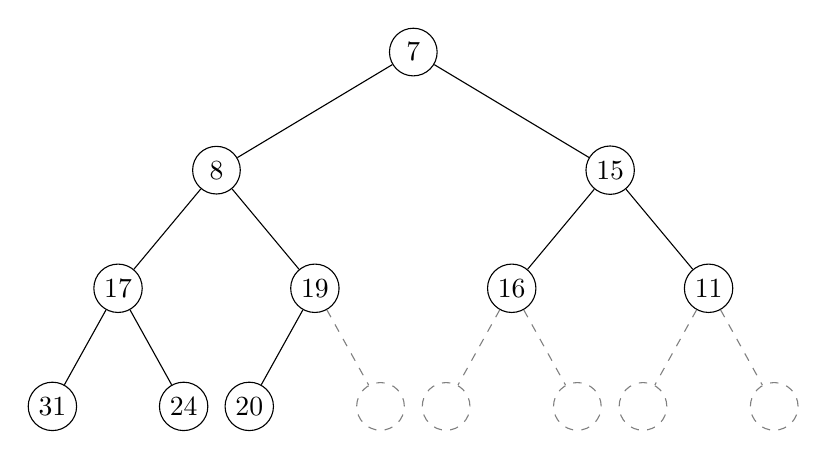
\begin{tikzpicture}[%level distance=5mm,
            inner sep=2pt,
            every node/.style={draw,circle,minimum size=4ex},
            level/.style = {sibling distance = 50mm/#1},
            ]
            
            \node {7}
                child {node {8}
                    child {node {17}
                        child {node {31}}
                        child {node {24}}
                    }
                    child {node {19}
                        child {node {20}}
                        child {node[dashed, color=gray] {} edge from parent[dashed, color=gray]}
                    }
                }
                child {node {15}
                    child {node {16}
                        child {node[dashed, color=gray] {} edge from parent[dashed, color=gray]}
                        child {node[dashed, color=gray] {} edge from parent[dashed, color=gray]}
                    }
                    child {node {11}
                        child {node[dashed, color=gray] {} edge from parent[dashed, color=gray]}
                        child {node[dashed, color=gray] {} edge from parent[dashed, color=gray]}
                    }
                };
        \end{tikzpicture}
    \end{center}
\end{frame}
\begin{frame}{Binary Heap \textsc{DeleteMin}}
    1. Return the root value, and replace the root node with the last element in the array.

    \begin{center}
        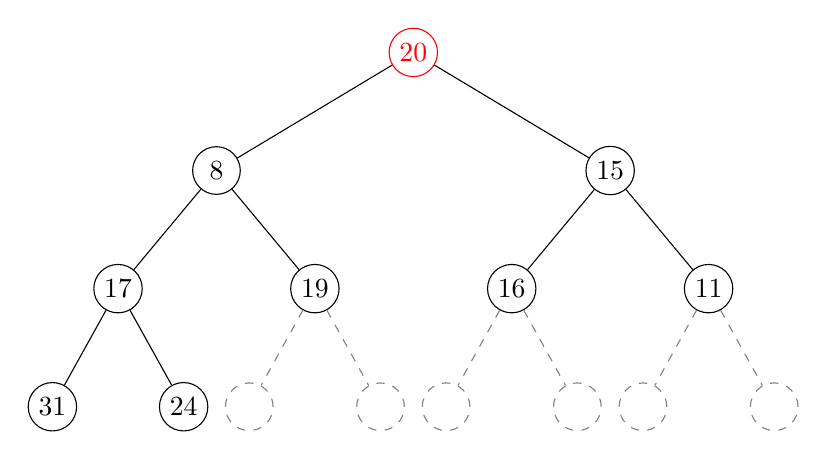
\begin{tikzpicture}[%level distance=5mm,
            inner sep=2pt,
            every node/.style={draw,circle,minimum size=4ex},
            level/.style = {sibling distance = 50mm/#1},
            ]
            
            \node[color=red] {20}
                child {node {8}
                    child {node {17}
                        child {node {31}}
                        child {node {24}}
                    }
                    child {node {19}
                        child {node[dashed, color=gray] {} edge from parent[dashed, color=gray]}
                        child {node[dashed, color=gray] {} edge from parent[dashed, color=gray]}
                    }
                }
                child {node {15}
                    child {node {16}
                        child {node[dashed, color=gray] {} edge from parent[dashed, color=gray]}
                        child {node[dashed, color=gray] {} edge from parent[dashed, color=gray]}
                    }
                    child {node {11}
                        child {node[dashed, color=gray] {} edge from parent[dashed, color=gray]}
                        child {node[dashed, color=gray] {} edge from parent[dashed, color=gray]}
                    }
                };
        \end{tikzpicture}
    \end{center}
\end{frame}
\begin{frame}{Binary Heap \textsc{DeleteMin}}
    2. Swap with smallest child until both children are larger.

    \begin{center}
        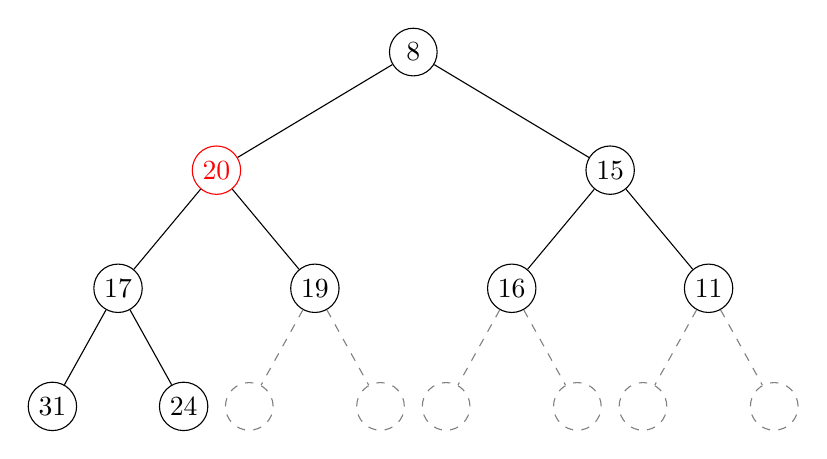
\begin{tikzpicture}[%level distance=5mm,
            inner sep=2pt,
            every node/.style={draw,circle,minimum size=4ex},
            level/.style = {sibling distance = 50mm/#1},
            ]
            
            \node {8}
                child {node[color=red] {20}
                    child {node {17}
                        child {node {31}}
                        child {node {24}}
                    }
                    child {node {19}
                        child {node[dashed, color=gray] {} edge from parent[dashed, color=gray]}
                        child {node[dashed, color=gray] {} edge from parent[dashed, color=gray]}
                    }
                }
                child {node {15}
                    child {node {16}
                        child {node[dashed, color=gray] {} edge from parent[dashed, color=gray]}
                        child {node[dashed, color=gray] {} edge from parent[dashed, color=gray]}
                    }
                    child {node {11}
                        child {node[dashed, color=gray] {} edge from parent[dashed, color=gray]}
                        child {node[dashed, color=gray] {} edge from parent[dashed, color=gray]}
                    }
                };
        \end{tikzpicture}
    \end{center}
\end{frame}
\begin{frame}{Binary Heap \textsc{DeleteMin}}
    2. Swap with smallest child until both children are larger.

    \begin{center}
        \begin{tikzpicture}[%level distance=5mm,
            inner sep=2pt,
            every node/.style={draw,circle,minimum size=4ex},
            level/.style = {sibling distance = 50mm/#1},
            ]
            
            \node {8}
                child {node {17}
                    child {node[color=sigma@green] {20}
                        child {node {31}}
                        child {node {24}}
                    }
                    child {node {19}
                        child {node[dashed, color=gray] {} edge from parent[dashed, color=gray]}
                        child {node[dashed, color=gray] {} edge from parent[dashed, color=gray]}
                    }
                }
                child {node {15}
                    child {node {16}
                        child {node[dashed, color=gray] {} edge from parent[dashed, color=gray]}
                        child {node[dashed, color=gray] {} edge from parent[dashed, color=gray]}
                    }
                    child {node {11}
                        child {node[dashed, color=gray] {} edge from parent[dashed, color=gray]}
                        child {node[dashed, color=gray] {} edge from parent[dashed, color=gray]}
                    }
                };
        \end{tikzpicture}
    \end{center}
\end{frame}
\begin{frame}{Binary Heap \textsc{DeleteMin}}
    Worst case, the replacement value will be swapped all the way to the bottom. Because this is a binary tree, we know this is \textcolor{sigma@mainblue}{$O(\log n)$}.
\end{frame}


\begin{frame}{Binary Heap \textsc{DecreaseKey}}
    This is the same as insert: decrease the priority of the node, then swap it with its parent until the parent is larger: \textcolor{sigma@mainblue}{$O(\log n)$}.
\end{frame}


\begin{frame}{Binary vs. Fibonacci Heap Runtimes}
    \begin{center}
        \begin{tabular}{|c|c|c|}
            \hline
            & Binary Heap & Fibonacci Heap \\
            \hline
            \textsc{Insert} & \textcolor{sigma@mainblue}{$O(\log n)$} & \textcolor{sigma@mainblue}{$O(1)$} \\
            \textsc{FindMin} & \textcolor{sigma@mainblue}{$O(1)$} & \textcolor{sigma@mainblue}{$O(1)$}\\
            \textsc{DeleteMin} & \textcolor{sigma@mainblue}{$O(\log n)$} & \textcolor{sigma@mainblue}{$O(\log n)$} \\
            \textsc{DecreaseKey} & \textcolor{sigma@mainblue}{$O(\log n)$} & \textcolor{sigma@mainblue}{$O(1)$} \\
            \hline
        \end{tabular}
    \end{center}
\end{frame}


\begin{frame}{}
      \begin{center}
    {\color{sigma@mainblue} \LARGE Questions?}
  \end{center}
\end{frame}


\begin{frame}{Binomial Heaps}
    First step on the way to Fibonacci heaps: what if we use more than one tree?\pause
    
    Properties:
    \begin{itemize}
        \item Composed of a forest of trees.\pause
        \item Binomial tree of order $k$ is a node with $k$ children \textbf{that are themselves binomial trees} of orders $k - 1, k - 2, \ldots, 2, 1, 0$.\pause
        \item There can be at most one binomial tree for each order.\pause
        \item Level $\ell$ has $\binom{k}{\ell}$ nodes in a binomial tree of order $k$.\pause
        \item Thus, a tree of order $k$ has $2^k$ nodes.\pause
        \item Thus, the largest degree is bounded by \textcolor{sigma@mainblue}{$O(\log n)$}.
    \end{itemize}
\end{frame}

\begin{frame}{Binomial Heap Example}
    (All one heap, nodes labeled with their degree.)
    \begin{center}
        \begin{tikzpicture}[
            inner sep=2pt,
            every node/.style={draw,circle,minimum size=4ex},
            % level/.style = {sibling distance = 30mm/#1},
            ]
            
            \node {0};
            \node at (1.75, 0) {1}
                child {node[color=sigma@mainblue] {0}};
            \node at (4.5, 0) {2}
                child {node[color=sigma@mainblue] {1}
                    child {node[color=sigma@mainblue] {0} edge from parent[color=sigma@mainblue]}
                }
                child {node[color=red] {0}};
            \node at (9, 0) {3}
                child {node[color=sigma@mainblue] {2}
                    child {node[color=sigma@mainblue] {1}
                        edge from parent[color=sigma@mainblue]
                        child {node {0}}
                    }
                    child {node[color=sigma@mainblue] {0} edge from parent[color=sigma@mainblue]}
                }
                child {node[color=red] {1}
                    child {node[color=red] {0} edge from parent[color=red]}
                }
                child {node[color=sigma@green] {0}};
        \end{tikzpicture}
    \end{center}
\end{frame}

\begin{frame}{Binomial Heap Notes}
    \begin{itemize}
        \item Combining two binomial heaps of degree $d$ gives a binomial heap of degree $d + 1$:
        \begin{center}
        \begin{tikzpicture}[
            inner sep=2pt,
            every node/.style={draw,circle,minimum size=4ex},
            % level/.style = {sibling distance = 30mm/#1},
            ]
            
            \node[color=red] at (9, 0) {3}
                child {node[color=sigma@mainblue] {2}
                    child {node[color=sigma@mainblue] {1}
                        edge from parent[color=sigma@mainblue]
                        child {node {0}}
                    }
                    child {node[color=sigma@mainblue] {0} edge from parent[color=sigma@mainblue]}
                }
                child {node[color=red] {1}
                    edge from parent[color=red]
                    child {node[color=red] {0} edge from parent[color=red]}
                }
                child {node[color=red] {0} edge from parent[color=red]};
        \end{tikzpicture}
    \end{center}
    \end{itemize}
\end{frame}

\begin{frame}{Binomial Heap \textsc{Insert}}
    Using amortized analysis, a binomial heap can insert in \textcolor{sigma@mainblue}{$O(1)$} by adding a single node as a new tree.

    (More on amortized analysis in a moment.)
\end{frame}




\section{Fibonacci Heaps}
\frame{\sectionpage}

\begin{frame}{Fibonacci Heaps}
    Properties:
    \begin{itemize}
        \item Binomial heap that can have more than one tree of any degree.\pause
        \item We can remove at most one child from each node. (We mark nodes that have had a child removed) \pause
    \end{itemize}
    Very loose structure; could just be a list of all root nodes. We use amortized analysis to get the runtimes we want.
\end{frame}


\begin{frame}{Formalizing Amortized Analysis}
    \begin{itemize}
        \item We use amortized analysis when the work done by slow operations can be attributed evenly to a predictable number of fast operations.\pause
        \item With the $\emph{Potential Method}$, we ``bank'' time in a potential function, $\phi$, on the fast operations, then ``cash out'' on the slow operations.\pause
        \item Formally, we define $\Delta \phi_o$ as the change in potential after operation $o$. Then the amortized time is calculated as $$T_{\textit{amortized}}(o) = T_{\textit{actual}}(o) + C\cdot \Delta \phi_o$$ for a constant $C$ that disappears in big $O$.\pause
        \item When we ``cash out'', the amortized time is smaller than the actual time, and $\phi$ decreases (usually to $0$).
    \end{itemize}
\end{frame}


\begin{frame}{Amortizing a Fibonacci Heap}
    \begin{itemize}
        \item We define $\phi$ as $$\phi = t + 2m$$ for a Fibonacci heap with $t$ trees and $m$ marked nodes.
        \pause
        \item This looks really arbitrary, but we will soon see why it works. 
    \end{itemize}
\end{frame}


\begin{frame}{Fibonacci Heap \textsc{Insert}}
    \begin{itemize}
        \item To insert, we simply add a new tree to the heap with the node we are adding as the root.\pause
        \item We maintain a pointer to the minimum element, so if this is the new minimum, update the pointer.
        \item \textcolor{sigma@mainblue}{$O(1)$}.
    \end{itemize}
\end{frame}
\begin{frame}{Fibonacci Heap \textsc{Insert} Example}
    \begin{center}
        \begin{tikzpicture}[inner sep=2pt,
            every node/.style={draw,circle,minimum size=4ex},level/.append style={level distance=1cm}]
                \node(n23) at (-2.25, 0) {23}
                    child {node(n34) {34}}
                    child {
                        node(n48) {48}
                        child {node(n50) {50}}
                    };
                \node(n33) at (0, 0) {33};
                \node(n5) at (1.5, 0) {5}
                    child {node(n56) {56}};
                \node(n40) at (3, 0) {40};
                \node(n19) at (4.5, 0) {19};

            \begin{scope}[->, line width=1pt]
                \draw[->,line width=1pt](1.5, 1)--(n5);
            \end{scope}
            \pause
            \node[color=sigma@mainblue](n3) at (-4.5, 0) {3};
        \end{tikzpicture}
    \end{center}
\end{frame}
\begin{frame}{Fibonacci Heap \textsc{Insert} Example}
    \begin{center}
        \begin{tikzpicture}[inner sep=2pt,
            every node/.style={draw,circle,minimum size=4ex},level/.append style={level distance=1cm}]
                \node(n23) at (-2.25, 0) {23}
                    child {node(n34) {34}}
                    child {
                        node(n48) {48}
                        child {node(n50) {50}}
                    };
                \node(n33) at (0, 0) {33};
                \node(n5) at (1.5, 0) {5}
                    child {node(n56) {56}};
                \node(n40) at (3, 0) {40};
                \node(n19) at (4.5, 0) {19};

            \begin{scope}[->, line width=1pt]
                \draw[->,line width=1pt](-4.5, 1)--(n3);
            \end{scope}
            \node[color=sigma@mainblue](n3) at (-4.5, 0) {3};
        \end{tikzpicture}
    \end{center}
\end{frame}


\begin{frame}{Fibonacci Heap \textsc{FindMin}}
    Because we maintain a pointer to the minimum element, accessing it is \textcolor{sigma@mainblue}{$O(1)$}.
    \pause
    \begin{center}
        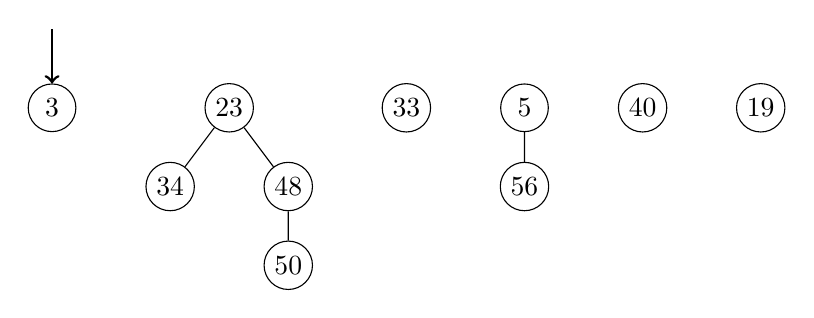
\begin{tikzpicture}[inner sep=2pt,
            every node/.style={draw,circle,minimum size=4ex},level/.append style={level distance=1cm}]
                \node(n3) at (-4.5, 0) {3};
                \node(n23) at (-2.25, 0) {23}
                    child {node(n34) {34}}
                    child {
                        node(n48) {48}
                        child {node(n50) {50}}
                    };
                \node(n33) at (0, 0) {33};
                \node(n5) at (1.5, 0) {5}
                    child {node(n56) {56}};
                \node(n40) at (3, 0) {40};
                \node(n19) at (4.5, 0) {19};

            \begin{scope}[->, line width=1pt]
                \draw[->,line width=1pt](-4.5, 1)--(n3);
            \end{scope}
        \end{tikzpicture}
    \end{center}
\end{frame}


\begin{frame}{Fibonacci Heap \textsc{DecreaseKey}}
    1. Decrease the key. If the new value maintains the heap property, we are done.

    \begin{center}
        \begin{tikzpicture}[
            inner sep=2pt,
            every node/.style={draw,circle,minimum size=4ex},
            % level/.style = {sibling distance = 30mm/#1},
            ]
            \node at (0, 0) {2}
                child {node {23}
                    child {node {40}
                        child {node {46}}
                    }
                    child {node {35}}
                }
                child {node{10}
                    child {node{22}}
                }
                child {node {7}};
            \node at (7, 0) {2}
                child {node {23}
                    child {node[color=sigma@mainblue] {29}
                        child {node {46}}
                    }
                    child {node {35}}
                }
                child {node{10}
                    child {node{22}}
                }
                child {node {7}};
            \begin{scope}[->, line width=1pt]
                \draw[->,line width=1pt](3, -2)--(4, -2);
            \end{scope}
        \end{tikzpicture}
    \end{center}
\end{frame}
\begin{frame}{Fibonacci Heap \textsc{DecreaseKey}}
    2. Otherwise, cut the decreased key (and its subtree) out into a new tree.

    \begin{center}
        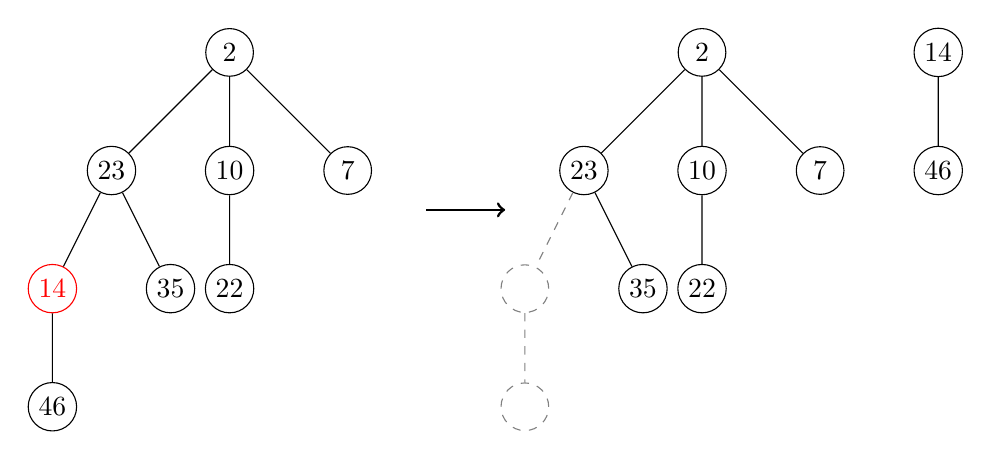
\begin{tikzpicture}[
            inner sep=2pt,
            every node/.style={draw,circle,minimum size=4ex},
            % level/.style = {sibling distance = 30mm/#1},
            ]
            \node at (0, 0) {2}
                child {node {23}
                    child {node[color=red] {14}
                        child {node {46}}
                    }
                    child {node {35}}
                }
                child {node{10}
                    child {node{22}}
                }
                child {node {7}};
            \node at (6, 0) {2}
                child {node {23}
                    child {node[dashed, color=gray] {} edge from parent[dashed, color=gray]
                        child {node[dashed, color=gray] {} edge from parent[dashed, color=gray]}
                    }
                    child {node {35}}
                }
                child {node{10}
                    child {node{22}}
                }
                child {node {7}};
            \node at (9, 0) {14}
                child {node {46}};
                
            \begin{scope}[->, line width=1pt]
                \draw[->,line width=1pt](2.5, -2)--(3.5, -2);
            \end{scope}
        \end{tikzpicture}
    \end{center}
\end{frame}
\begin{frame}{Fibonacci Heap \textsc{DecreaseKey}}
    3. If the parent was unmarked, mark it. Otherwise, cut it out, unmark it, and repeat for this node's parent.

    \begin{center}
        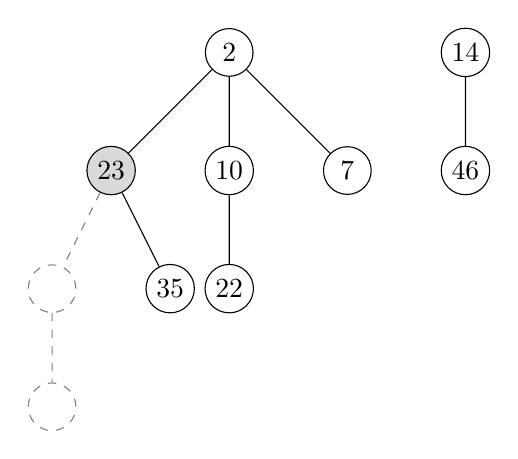
\begin{tikzpicture}[
            inner sep=2pt,
            every node/.style={draw,circle,minimum size=4ex},
            % level/.style = {sibling distance = 30mm/#1},
            ]
            \node at (6, 0) {2}
                child {node[fill=gray!30] {23}
                    child {node[dashed, color=gray] {} edge from parent[dashed, color=gray]
                        child {node[dashed, color=gray] {} edge from parent[dashed, color=gray]}
                    }
                    child {node {35}}
                }
                child {node{10}
                    child {node{22}}
                }
                child {node {7}};
            \node at (9, 0) {14}
                child {node {46}};
        \end{tikzpicture}
    \end{center}
\end{frame}
\begin{frame}{Fibonacci Heap \textsc{DecreaseKey}}
    Now, if we cut out $35$, we would also cut out $23$:
    
    \begin{center}
        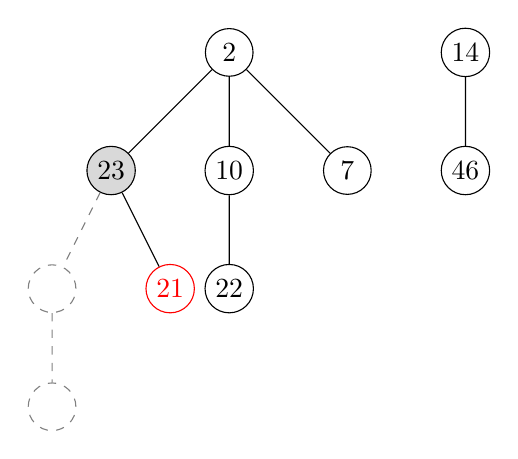
\begin{tikzpicture}[
            inner sep=2pt,
            every node/.style={draw,circle,minimum size=4ex},
            % level/.style = {sibling distance = 30mm/#1},
            ]
            \node at (6, 0) {2}
                child {node[fill=gray!30] {23}
                    child {node[dashed, color=gray] {} edge from parent[dashed, color=gray]
                        child {node[dashed, color=gray] {} edge from parent[dashed, color=gray]}
                    }
                    child {node[color=red] {21}}
                }
                child {node{10}
                    child {node{22}}
                }
                child {node {7}};
            \node at (9, 0) {14}
                child {node {46}};
        \end{tikzpicture}
    \end{center}
\end{frame}
\begin{frame}{Fibonacci Heap \textsc{DecreaseKey}}
    Now, if we cut out $35$, we would also cut out $23$:
    
    \begin{center}
        \begin{tikzpicture}[
            inner sep=2pt,
            every node/.style={draw,circle,minimum size=4ex},
            % level/.style = {sibling distance = 30mm/#1},
            ]
            \node at (6, 0) {2}
                child {node[dashed, color=gray] {} edge from parent[dashed, color=gray]
                    child {node[dashed, color=gray] {} edge from parent[dashed, color=gray]
                        child {node[dashed, color=gray] {} edge from parent[dashed, color=gray]}
                    }
                    child {node {}}
                }
                child {node{10}
                    child {node{22}}
                }
                child {node {7}};
            \node at (9, 0) {14}
                child {node {46}};
            \node at (10.5, 0) {21};
            \node at (12, 0) {23};
        \end{tikzpicture}
    \end{center}
\end{frame}
\begin{frame}{Fibonacci Heap \textsc{DecreaseKey} Analysis}
    \begin{itemize}
        \item Suppose we made $k$ cuts in total. Then we added $k$ trees in \textcolor{sigma@mainblue}{$O(k)$}.\pause
        \item Of all the nodes we cut out, only the first was unmarked, but all are unmarked now. Including the final extra node we marked, we have that marked nodes changed by $-(k - 1) + 1 = -k + 2$.\pause
        \item Remember $\phi = t + 2m$ for $t$ trees and $m$ marked nodes, and $T_{\textit{amortized}}(o) = T_{\textit{actual}}(o) + C \cdot \Delta \phi$.\pause
        \item Thus, $\Delta \phi = k + 2(-k + 2) = -k + 4$.\pause
        \item So our amortized time is \textcolor{sigma@mainblue}{$O(1)$}.\pause
        \item Notice our choice of $\phi$ was important here.
    \end{itemize}
\end{frame}


\begin{frame}{Fibonacci Heap \textsc{DeleteMin} Phase 1}
    Cut out the minimum node (which must be a root) and make its children roots of new trees.

    \begin{center}
        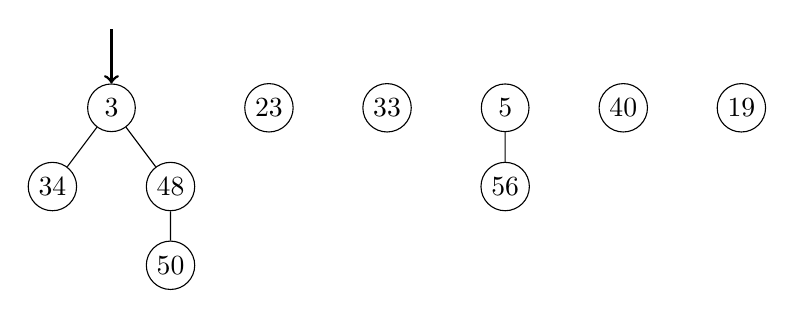
\begin{tikzpicture}[inner sep=2pt,
            every node/.style={draw,circle,minimum size=4ex},level/.append style={level distance=1cm}]
                \node(n23) at (-1.5, 0) {23};
                \node(n3) at (-3.5, 0) {3}
                    child {node(n34) {34}}
                    child {
                        node(n48) {48}
                        child {node(n50) {50}}
                    };
                \node(n33) at (0, 0) {33};
                \node(n5) at (1.5, 0) {5}
                    child {node(n56) {56}};
                \node(n40) at (3, 0) {40};
                \node(n19) at (4.5, 0) {19};

            \begin{scope}[->, line width=1pt]
                \draw[->,line width=1pt](-3.5, 1)--(n3);
            \end{scope}
        \end{tikzpicture}
    \end{center}
\end{frame}
\begin{frame}{Fibonacci Heap \textsc{DeleteMin} Phase 1}
    Cut out the minimum node (which must be a root) and make its children roots of new trees.

    \begin{center}
        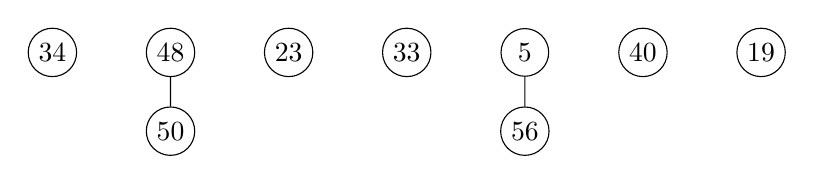
\begin{tikzpicture}[inner sep=2pt,
            every node/.style={draw,circle,minimum size=4ex},level/.append style={level distance=1cm}]
                \node(n23) at (-1.5, 0) {23};
                \node(n34) at (-4.5, 0) {34};
                \node(n48) at (-3, 0) {48}
                    child {node(n50) {50}};
                \node(n33) at (0, 0) {33};
                \node(n5) at (1.5, 0) {5}
                    child {node(n56) {56}};
                \node(n40) at (3, 0) {40};
                \node(n19) at (4.5, 0) {19};
        \end{tikzpicture}
    \end{center}

    \pause
    With $d$ children, this operation is \textcolor{sigma@mainblue}{$O(d)$}. We will see later that \textcolor{sigma@mainblue}{$O(d)$} $=$ \textcolor{sigma@mainblue}{$O(\log n)$} for a fibonacci heap with $n$ nodes. 
\end{frame}

\begin{frame}{Fibonacci Heap \textsc{DeleteMin} Phase 2}
    \begin{itemize}
        \item Now we need to update the minimum pointer.\pause
        \item Until now, we haven't enforced much structure, so in general, there might now be $n$ roots, and finding the minimum is \textcolor{sigma@mainblue}{$O(n)$}.\pause
        \item However, if we ``clean up,'' future calls to \textsc{DeleteMin} could be faster, and could give us a $\Delta \phi$ that helps in amortized analysis.\pause
        \item Like the last slide, I will assume the largest degree of any root is \textcolor{sigma@mainblue}{$O(\log n)$}, and prove this later.
    \end{itemize}
\end{frame}
\begin{frame}{Fibonacci Heap \textsc{DeleteMin} Phase 2}
    1. Create an array of length \textcolor{sigma@mainblue}{$O(\log n)$} to track trees of every possible degree.

    \begin{center}
        \begin{tikzpicture}
            \begin{scope}[local bounding box=scope1]
                \matrix[matrix of nodes, ampersand replacement=\&, nodes={draw, minimum width=0.5cm, minimum height=0.5cm}] (array)
                {
                    \node(a0){0}; \& \node(a1){1}; \& \node(a2){2}; \& \node(a3){3}; \\
                };
            \end{scope}

            \begin{scope}[shift={($(scope1.south)+(0,-1cm)$)},inner sep=2pt,
            every node/.style={draw,circle,minimum size=4ex},level/.append style={level distance=1cm}]
                \node(n3) at (-4.5, 0) {3};
                \node(n23) at (-2.25, 0) {23}
                    child {node(n34) {34}}
                    child {
                        node(n48) {48}
                        child {node(n50) {50}}
                    };
                \node(n33) at (0, 0) {33}
                    child {node(n35) {35}};
                \node(n5) at (1.5, 0) {5}
                    child {node(n56) {56}};
                \node(n40) at (3, 0) {40}
                    child {node(n45) {45}};
                \node(n19) at (4.5, 0) {19};
            \end{scope}

            \begin{scope}[->, line width=1pt]
                % \draw[->,line width=1pt](a1.south)--(n23);
            \end{scope}
        \end{tikzpicture}
    \end{center}
\end{frame}
\begin{frame}{Fibonacci Heap \textsc{DeleteMin} Phase 2}
    2. Put each tree into an index of the array. If there is already a tree there, merge them to create a tree of degree $+ 1$.

    \begin{center}
        \begin{tikzpicture}
            \begin{scope}[local bounding box=scope1]
                \matrix[matrix of nodes, ampersand replacement=\&, nodes={draw, minimum width=0.5cm, minimum height=0.5cm}] (array)
                {
                    \node(a0){0}; \& \node(a1){1}; \& \node(a2){2}; \& \node(a3){3}; \\
                };
            \end{scope}

            \begin{scope}[shift={($(scope1.south)+(0,-1cm)$)},inner sep=2pt,
            every node/.style={draw,circle,minimum size=4ex},level/.append style={level distance=1cm}]
                \node(n3) at (-4.5, 0) {3};
                \node(n23) at (-2.25, 0) {23}
                    child {node(n34) {34}}
                    child {
                        node(n48) {48}
                        child {node(n50) {50}}
                    };
                \node(n33) at (0, 0) {33}
                    child {node(n35) {35}};
                \node(n5) at (1.5, 0) {5}
                    child {node(n56) {56}};
                \node(n40) at (3, 0) {40}
                    child {node(n45) {45}};
                \node(n19) at (4.5, 0) {19};
            \end{scope}

            \begin{scope}[->, line width=1pt]
                \draw(a0.south)--(n3);
                \pause
                \draw(a2.south)--(n23);
                \pause
                \draw(a1.south)--(n33);
                \pause
                \draw[red](a1.south)--(n5);
            \end{scope}
        \end{tikzpicture}
    \end{center}
\end{frame}
\begin{frame}{Fibonacci Heap \textsc{DeleteMin} Phase 2}
    2. Put each tree into an index of the array. If there is already a tree there, merge them to create a tree of degree $+ 1$.

    \begin{center}
        \begin{tikzpicture}
            \begin{scope}[local bounding box=scope1]
                \matrix[matrix of nodes, ampersand replacement=\&, nodes={draw, minimum width=0.5cm, minimum height=0.5cm}] (array)
                {
                    \node(a0){0}; \& \node(a1){1}; \& \node(a2){2}; \& \node(a3){3}; \\
                };
            \end{scope}

            \begin{scope}[shift={($(scope1.south)+(0,-1cm)$)},inner sep=2pt,
            every node/.style={draw,circle,minimum size=4ex},level/.append style={level distance=1cm}]
                \node(n3) at (-4.5, 0) {3};
                \node(n23) at (-2.25, 0) {23}
                    child {node(n34) {34}}
                    child {
                        node(n48) {48}
                        child {node(n50) {50}}
                    };
                \node[color=red](n5) at (0.75, 0) {5}
                    child {node[color=red](n56) {56} edge from parent[color=red]}
                    child {
                        node[color=sigma@mainblue](n33) {33}
                        child {node[color=sigma@mainblue](n35) {35} edge from parent[color=sigma@mainblue]}
                    };
                \node(n40) at (3, 0) {40}
                    child {node(n45) {45}};
                \node(n19) at (4.5, 0) {19};
            \end{scope}

            \begin{scope}[->, line width=1pt]
                \draw(a0.south)--(n3);
                \draw(a2.south)--(n23);
                \pause
                \draw[red](a2.south)--(n5);
            \end{scope}
        \end{tikzpicture}
    \end{center}
\end{frame}
\begin{frame}{Fibonacci Heap \textsc{DeleteMin} Phase 2}
    2. Put each tree into an index of the array. If there is already a tree there, merge them to create a tree of degree $+ 1$.

    \begin{center}
        \begin{tikzpicture}
            \begin{scope}[local bounding box=scope1]
                \matrix[matrix of nodes, ampersand replacement=\&, nodes={draw, minimum width=0.5cm, minimum height=0.5cm}] (array)
                {
                    \node(a0){0}; \& \node(a1){1}; \& \node(a2){2}; \& \node(a3){3}; \\
                };
            \end{scope}

            \begin{scope}[shift={($(scope1.south)+(0,-1cm)$)},inner sep=2pt,
            every node/.style={draw,circle,minimum size=4ex},level/.append style={level distance=1cm}]
                \node(n3) at (-4.5, 0) {3};
                \node[color=red](n5) at (-1.5, 0) {5}
                    child {node[color=red](n56) {56} edge from parent[color=red]}
                    child {
                        node[color=red](n33) {33}
                        edge from parent[color=red]
                        child {node[color=red](n35) {35} edge from parent[color=red]}
                    }
                    child {
                        node[color=sigma@mainblue](n23) at (0.75, 0) {23}
                        child {node[color=sigma@mainblue](n34) {34} edge from parent[color=sigma@mainblue]}
                        child {
                            node[color=sigma@mainblue](n48) {48}
                            edge from parent[color=sigma@mainblue]
                            child {node[color=sigma@mainblue](n50) {50} edge from parent[color=sigma@mainblue]}
                        }
                    };
                \node(n40) at (3, 0) {40}
                    child {node(n45) {45}};
                \node(n19) at (4.5, 0) {19};
            \end{scope}

            \begin{scope}[->, line width=1pt]
                \draw(a0.south)--(n3);
                \pause
                \draw(a3.south)--(n5);
            \end{scope}
        \end{tikzpicture}
    \end{center}
\end{frame}
\begin{frame}{Fibonacci Heap \textsc{DeleteMin} Phase 2}
    2. Put each tree into an index of the array. If there is already a tree there, merge them to create a tree of degree $+ 1$.

    \begin{center}
        \begin{tikzpicture}
            \begin{scope}[local bounding box=scope1]
                \matrix[matrix of nodes, ampersand replacement=\&, nodes={draw, minimum width=0.5cm, minimum height=0.5cm}] (array)
                {
                    \node(a0){0}; \& \node(a1){1}; \& \node(a2){2}; \& \node(a3){3}; \\
                };
            \end{scope}

            \begin{scope}[shift={($(scope1.south)+(0,-1cm)$)},inner sep=2pt,
            every node/.style={draw,circle,minimum size=4ex},level/.append style={level distance=1cm}]
                \node(n3) at (-4.5, 0) {3};
                \node(n5) at (-1.5, 0) {5}
                    child {node(n56) {56}}
                    child {
                        node(n33) {33}
                        child {node(n35) {35}}
                    }
                    child {
                        node(n23) at (0.75, 0) {23}
                        child {node(n34) {34}}
                        child {
                            node(n48) {48}
                            child {node(n50) {50}}
                        }
                    };
                \node(n40) at (3, 0) {40}
                    child {node(n45) {45}};
                \node(n19) at (4.5, 0) {19};
            \end{scope}

            \begin{scope}[->, line width=1pt]
                \draw(a0.south)--(n3);
                \draw(a3.south)--(n5);
                \draw(a1.south)--(n40);
                \pause
                \draw[red](a0.south)--(n19);
            \end{scope}
        \end{tikzpicture}
    \end{center}
\end{frame}
\begin{frame}{Fibonacci Heap \textsc{DeleteMin} Phase 2}
    2. Put each tree into an index of the array. If there is already a tree there, merge them to create a tree of degree $+ 1$.

    \begin{center}
        \begin{tikzpicture}
            \begin{scope}[local bounding box=scope1]
                \matrix[matrix of nodes, ampersand replacement=\&, nodes={draw, minimum width=0.5cm, minimum height=0.5cm}] (array)
                {
                    \node(a0){0}; \& \node(a1){1}; \& \node(a2){2}; \& \node(a3){3}; \\
                };
            \end{scope}

            \begin{scope}[shift={($(scope1.south)+(0,-1cm)$)},inner sep=2pt,
            every node/.style={draw,circle,minimum size=4ex},level/.append style={level distance=1cm}]
                \node[color=sigma@mainblue](n3) at (-3.75, 0) {3}
                    child {node[color=red](n19) {19}};
                \node(n5) at (-0.75, 0) {5}
                    child {node(n56) {56}}
                    child {
                        node(n33) {33}
                        child {node(n35) {35}}
                    }
                    child {
                        node(n23) at (0.75, 0) {23}
                        child {node(n34) {34}}
                        child {
                            node(n48) {48}
                            child {node(n50) {50}}
                        }
                    };
                \node(n40) at (3.75, 0) {40}
                    child {node(n45) {45}};
            \end{scope}

            \begin{scope}[->, line width=1pt]
                \draw(a3.south)--(n5);
                \draw(a1.south)--(n40);
                \pause
                \draw[red](a1.south)--(n3);
            \end{scope}
        \end{tikzpicture}
    \end{center}
\end{frame}
\begin{frame}{Fibonacci Heap \textsc{DeleteMin} Phase 2}
    2. Put each tree into an index of the array. If there is already a tree there, merge them to create a tree of degree $+ 1$.

    \begin{center}
        \begin{tikzpicture}
            \begin{scope}[local bounding box=scope1]
                \matrix[matrix of nodes, ampersand replacement=\&, nodes={draw, minimum width=0.5cm, minimum height=0.5cm}] (array)
                {
                    \node(a0){0}; \& \node(a1){1}; \& \node(a2){2}; \& \node(a3){3}; \\
                };
            \end{scope}

            \begin{scope}[shift={($(scope1.south)+(0,-1cm)$)},inner sep=2pt,
            every node/.style={draw,circle,minimum size=4ex},level/.append style={level distance=1cm}]
                \node[color=red](n3) at (-3, 0) {3}
                    child {node[color=red](n19) {19} edge from parent[color=red]}
                    child {
                        node[color=sigma@mainblue](n40) {40}
                        child {node[color=sigma@mainblue](n45) {45} edge from parent[color=sigma@mainblue]}
                    };
                \node(n5) at (1, 0) {5}
                    child {node(n56) {56}}
                    child {
                        node(n33) {33}
                        child {node(n35) {35}}
                    }
                    child {
                        node(n23) at (0.75, 0) {23}
                        child {node(n34) {34}}
                        child {
                            node(n48) {48}
                            child {node(n50) {50}}
                        }
                    };
            \end{scope}

            \begin{scope}[->, line width=1pt]
                \draw(a3.south)--(n5);
                \pause
                \draw(a2.south)--(n3);
            \end{scope}
        \end{tikzpicture}
    \end{center}
\end{frame}

\begin{frame}{Fibonacci Heap \textsc{DeleteMin} Phase 2 Analysis}
    \begin{itemize}
        \item We need to allocate the array and visit each of $m$ starting roots for \textcolor{sigma@mainblue}{$O(\log n + m)$} actual runtime.\pause
        \item $\Delta \phi = \Delta(\# trees) = \textcolor{sigma@mainblue}{O(\log n) - m}$. (final - initial)\pause
        \item Thus, the amortized runtime for this phase is
        \begin{align*}
            \onslide<+->{&O(\log n + m) + C\cdot\big(O(\log n) - m\big) \\}
            \onslide<+->{&= O(\log\ n) + O(m) + C\cdot O(\log n) - C\cdot m \\}
            \onslide<+->{&= O(\log n) \quad\quad\quad\quad\text{(with large enough } C \text{)}}
        \end{align*}
    \end{itemize}
\end{frame}


\begin{frame}{Fibonacci Heap \textsc{DeleteMin} Phase 3}
    Find the minimum of the \textcolor{sigma@mainblue}{$O(\log n )$} roots that remain in \textcolor{sigma@mainblue}{$O(\log n )$} time.
    
    \begin{center}
        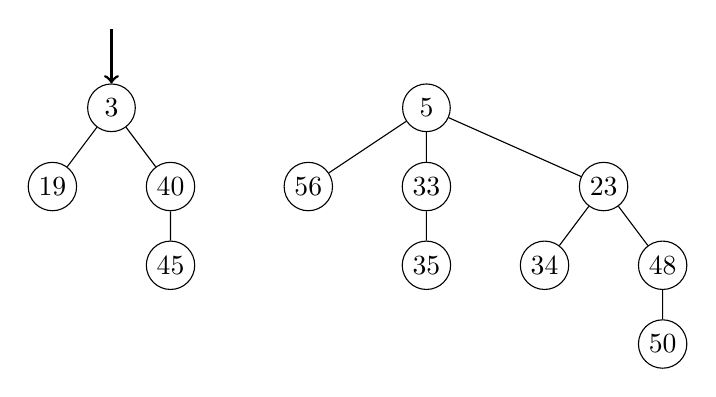
\begin{tikzpicture}[inner sep=2pt,
            every node/.style={draw,circle,minimum size=4ex},level/.append style={level distance=1cm}]
            \node(n3) at (-3, 0) {3}
                child {node(n19) {19}}
                child {
                    node(n40) {40}
                    child {node(n45) {45}}
                };
            \node(n5) at (1, 0) {5}
                child {node(n56) {56}}
                child {
                    node(n33) {33}
                    child {node(n35) {35}}
                }
                child {
                    node(n23) at (0.75, 0) {23}
                    child {node(n34) {34}}
                    child {
                        node(n48) {48}
                        child {node(n50) {50}}
                    }
                };
                
            \begin{scope}[->, line width=1pt]
                \draw(-3, 1)--(n3);
            \end{scope}
        \end{tikzpicture}
    \end{center}
\end{frame}


\begin{frame}{Fibonacci Heap \textsc{DeleteMin} Recap}
    Of all 3 phases, the slowest runtime was $O(\log\ n)$, so the overall runtime is \textcolor{sigma@mainblue}{$O(\log n )$}.
\end{frame}


\begin{frame}{}
      \begin{center}
    {\color{sigma@mainblue} \LARGE Questions?}
  \end{center}
\end{frame}


\begin{frame}{Fibonacci Heap Degree Bound Proof}
    \begin{itemize}
        \item Earlier, we assumed that the largest degree of any root is \textcolor{sigma@mainblue}{$O(\log n )$}. How do we know? This is where Fibonacci comes in.\pause
        \item We focus on one tree with degree $d$ and $n$ nodes total. We want
        \begin{align*}
            \onslide<+->{d & \le O(\log{n}) \\}
            \onslide<+->{d & \le \log_a{n} & \text{(for some $a > 1$)}\\}
            \onslide<+->{d \cdot \log{a} & \le  \log{n} & \text{(if } a \le 1 \text{, the } \le \text{ would flip)} \\}
            \onslide<+->{\log{a^d} & \le \log{n} \\}
            \onslide<+->{a^d & \le n}
        \end{align*}
        % \pause
        \onslide<+->{\item Thus, we need to show that $n$ grows exponentially with respect to $d$.}
    \end{itemize}
\end{frame}
\begin{frame}{Fibonacci Heap Degree Bound Proof}
    \begin{itemize}
        \item To do this, let's look for a lower bound on $n$ for a given $d$.\pause
        \item Consider a tree of degree $4$:
        \begin{center}
            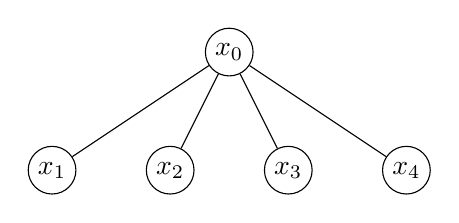
\begin{tikzpicture}[inner sep=2pt,
                every node/.style={draw,circle,minimum size=4ex}]
                \node {$x_0$}
                    child {node {$x_1$}}
                    child {node {$x_2$}}
                    child {node {$x_3$}}
                    child {node {$x_4$}};
            \end{tikzpicture}
        \end{center}\pause
        \item When $x_3$ was added, it must have been degree $2$.\pause
        \item Because each node can have at most one child removed, $x_3$ must now have degree at least $1$. Similarly, $x_4$ must have degree at least $2$.\pause
        \item In general, the $i^{th}$ child must have degree at least $i - 2$.
    \end{itemize}
\end{frame}
\begin{frame}{Fibonacci Heap Degree Bound Proof}
    \begin{itemize}
        \item We can use this to build up the minimum trees for each degree.\pause
        \item Minimum for degrees $0$ and $1$ (base cases) are trivial:
        \begin{center}
            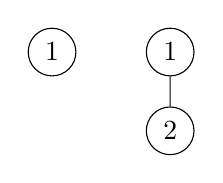
\begin{tikzpicture}[inner sep=2pt, every node/.style={draw,circle,minimum size=4ex}, level/.append style={level distance=1cm}]
                \node at (-0.75, 0) {1};
                \node at (0.75, 0) {1}
                    child {node {2}};
            \end{tikzpicture}
        \end{center}
    \end{itemize}
\end{frame}
\begin{frame}{Fibonacci Heap Degree Bound Proof}
    \begin{itemize}
        \item Then for tree of degree $d$ we can add tree of degree $d - 2$ as a child of tree $d - 1$.\pause
        \item Degrees $2$–$4$ are as follows:
        \begin{center}
            \begin{tikzpicture}[inner sep=2pt, every node/.style={draw,circle,minimum size=4ex}, level/.append style={level distance=1cm}, level/.style={sibling distance=10mm}]
                \node[color=sigma@mainblue] at (-5, 0) {1}
                    child {node[color=sigma@mainblue] {2} edge from parent[color=sigma@mainblue]}
                    child {node[color=red] {3}};\pause
                \node[color=sigma@mainblue] at (-1.875, 0) {1}
                    child {node[color=sigma@mainblue] {2} edge from parent[color=sigma@mainblue]}
                    child {node[color=sigma@mainblue] {3} edge from parent[color=sigma@mainblue]}
                    child {
                        node[color=red] {4}
                        child {node[color=red] {5} edge from parent[color=red]}
                    };\pause
                \node[color=sigma@mainblue] at (2.5, 0) {1}
                    child {node[color=sigma@mainblue] {2} edge from parent[color=sigma@mainblue]}
                    child {node[color=sigma@mainblue] {3} edge from parent[color=sigma@mainblue]}
                    child {
                        node[color=sigma@mainblue] {4} edge from parent[color=sigma@mainblue]
                        child {node[color=sigma@mainblue] {5} edge from parent[color=sigma@mainblue]}
                    }
                    child {
                        node[color=red] at (0.7, 0) {6}
                        child {node[color=red] {7} edge from parent[color=red]}
                        child {node[color=red] {8} edge from parent[color=red]; 5}
                    };
            \end{tikzpicture}
        \end{center}
    \end{itemize}
\end{frame}
\begin{frame}{Fibonacci Heap Degree Bound Proof}
    \begin{itemize}
        \item Fibonacci!
            \begin{center}
                \begin{tikzpicture}[inner sep=2pt, every node/.style={draw,circle,minimum size=4ex}, level/.append style={level distance=1cm}, level/.style={sibling distance=10mm}]
                    \node[opacity=0.35,text opacity=0.35,fill=black!10] at (-6.5, 0) {0};
                    \node[opacity=0.35,text opacity=0.35,fill=black!10] at (-5, 0) {1};
                    \node[fill=sigma@mainblue!30] at (-3.5, 0) {1};
                    \node at (-2, 0) {1}
                        child {node[fill=sigma@mainblue!30] {2}};
                    \node at (0, 0) {1}
                        child {node {2}}
                        child {node[fill=sigma@mainblue!30] {3}};
                    \node at (3, 0) {1}
                        child {node {2}}
                        child {node {3}}
                        child {
                            node {4}
                            child {node[fill=sigma@mainblue!30] {5}}
                        };
                \end{tikzpicture}
            \end{center}\pause
        \item We know that the growth of Fibonacci approaches $\Phi \approx 1.618$, so $n \ge \Phi^d$. which satisfies our goal.
    \end{itemize}
\end{frame}


\begin{frame}{Recap}
    \begin{center}
        \begin{tabular}{|c|c|c|c|}
            \hline
            & Binary Heap & Binomial Heap & Fibonacci Heap\\
            \hline
            \textsc{Insert} & \textcolor{sigma@mainblue}{$O(\log n )$} & \textcolor{sigma@mainblue}{$O(1)$} & \textcolor{sigma@mainblue}{$O(1)$} \\
            \textsc{FindMin} & \textcolor{sigma@mainblue}{$O(1)$} & \textcolor{sigma@mainblue}{$O(1)$} & \textcolor{sigma@mainblue}{$O(1)$} \\
            \textsc{DeleteMin} & \textcolor{sigma@mainblue}{$O(\log n )$} & \textcolor{sigma@mainblue}{$O(\log n )$} & \textcolor{sigma@mainblue}{$O(\log n )$} \\
            \textsc{DecreaseKey} & \textcolor{sigma@mainblue}{$O(\log n )$}& \textcolor{sigma@mainblue}{$O(\log n )$} & \textcolor{sigma@mainblue}{$O(1)$} \\
            \hline
        \end{tabular}
    \end{center}
\end{frame}


\begin{frame}{In practice...}
    \begin{itemize}
        \item Fibonacci heaps are usually implemented with pointers from parent to child, child to parent, and circularly between siblings.\pause
        \item This leads to large big-O constants and heavy reliance on pointers that gives much worse cache performance than binary heaps.\pause
        \item So, Fibonacci heaps are not often used, because they are too slow in practice.\pause
        \item Fibonacci heaps can still be faster for really large amounts of data.
    \end{itemize}
\end{frame}


\begin{frame}{}
      \begin{center}
    {\color{sigma@mainblue} \LARGE Questions?}
  \end{center}
\end{frame}


% Quotes are fun, find some to use!
\font\eightss=cmssq8
\font\eightssi=cmssqi8
\newcommand\quoteAuthorDate[3]{\begingroup
  \baselineskip 10pt
  \parfillskip 0pt
  \interlinepenalty 10000 % not needed in example
  \leftskip 0pt plus 40pc minus \parindent
  \let\rm=\eightss
  \let\sl=\eightssi
  \everypar{\sl}#1\par
  \nobreak\smallskip
  \noindent\rm--- #2\unskip\enspace(#3)\par
  \endgroup}
% If someone can figure out how to horizontally center this and make the text bigger that'd be cool
\begin{frame}
    \begin{center}
        \item \quoteAuthorDate{Computers are useless. They only give you the answers.}{Pablo Picasso}{\textcolor{sigma@mainblue}{1979}}
    \end{center}
\end{frame}

% Remove this slide if you came up with all the material yourself
\begin{frame}[allowframebreaks]{Bibliography}
    \bibliography{refs}
    \bibliographystyle{alpha}
     Wikimedia Foundation. (2024, January 17). \textit{Fibonacci heap}. Wikipedia. \url{https://en.wikipedia.org/wiki/Fibonacci_heap}
\end{frame}

\end{document}